\section{Resultados}

Este tópico é dedicado a apresentar os resultados, adversidades e contribuições 
alcançadas durante o desenvolvimento do estudo referente ao problema proposto. 
Por fim, são apresentadas considerações sobre as limitações ocorridas no 
desenvolvimento deste trabalho.

\subsection{Configuração do experimento}

Dada a matriz de referência \cite{matriz_referencia_redacao:2016}, a 
competência II foi selecionada aleatóriamente como o alvo da inferência 
indutiva dos classificadores. 

Para avaliar e validar a hipótese proposta, foram gerados resultados sobre dois 
\textit{datasets} extraidos de fontes diferentes, respectivamente (A, B).
Dentre as inúmeras possibilidades, não houve variação dos parâmetros de 
inferência indutiva dos classificadores, a fim, validar a hipótese de recuperar 
um padrão na valoração de uma redação, isto é, um dos classificadores, 
conjuntamente o mesmo, deve apresentar métricas de desempenho relevantes em 
ambos os \textit{datasets}.

\subsection{\textit{Datasets} \textbf{A} e \textbf{B}}

No caso dos \textit{datasets}, ambos dispõe da mesma quantidade de redações, com 
temas diversificados e passaram por um processo de avaliação manual com 
diferentes avaliadores. O \textit{dataset} \textbf{A} é constituído de 250 
redações, igual ao \textbf{B}. Os gráficos 
\ref{graphic:class_dataset_balanced_a} e \ref{graphic:class_dataset_balanced_b} 
demonstram a disposição das classes distintas (0.00, 0.50, 1.00, 1.50, 2.00) 
sobre a competência II, respectivamente de (\textbf{A}, \textbf{B}).

\pgfplotstableread[row sep=\\,col sep=&]{
    class & score  \\
    0.00  & 50 \\
    0.50  & 50 \\
    1.00  & 50 \\
    1.50  & 50 \\
    2.00  & 50  \\
    }\datasetAall

\begin{figure}[H]
\begin{center}
\begin{tikzpicture}
    \begin{axis}[
            ybar,
            width=8cm,
            height=7cm,
            symbolic x coords={0.00,0.50,1.00,1.50,2.00},
            bar width=10pt,
            ylabel=Quantidade,
            xlabel=Classes,
            xtick=data,
            axis lines*=left,
        ]
        \addplot[draw=black, fill=white] table[x=class,y=score]{\datasetAall};
        \node [above] at (axis cs:  0.00,50) {50};
        \node [above] at (axis cs:  0.50,50) {50};
        \node [above] at (axis cs:  1.00,50) {50};
        \node [above] at (axis cs:  1.50,50) {50};
        \node [above] at (axis cs:  2.00,50) {50};
    \end{axis}
\end{tikzpicture}
\caption{Distribuição das classes sobre a competência II de 250 redações do 
\textit{dataset} \textbf{A}.}
\label{graphic:class_dataset_balanced_a}
\end{center}
\end{figure}

\pgfplotstableread[row sep=\\,col sep=&]{
    class & score  \\
    0.00  & 50 \\
    0.50  & 50 \\
    1.00  & 50 \\
    1.50  & 50 \\
    2.00  & 50  \\
    }\datasetBall

\begin{figure}[H]
\begin{center}
\begin{tikzpicture}
    \begin{axis}[
            ybar,
            width=8cm,
            height=7cm,
            symbolic x coords={0.00,0.50,1.00,1.50,2.00},
            bar width=10pt,
            ylabel=Quantidade,
            xlabel=Classes,
            xtick=data,
            axis lines*=left,
        ]
        \addplot[draw=black, fill=white] table[x=class,y=score]{\datasetBall};
        \node [above] at (axis cs:  0.00,50) {50};
        \node [above] at (axis cs:  0.50,50) {50};
        \node [above] at (axis cs:  1.00,50) {50};
        \node [above] at (axis cs:  1.50,50) {50};
        \node [above] at (axis cs:  2.00,50) {50};
    \end{axis}
\end{tikzpicture}
\caption{Distribuição das classes sobre a competência II de 250 redações do 
\textit{dataset} \textbf{B}}
\label{graphic:class_dataset_balanced_b}
\end{center}
\end{figure}

Cada \textit{dataset} utilizado na indução foi fracionado em duas partes, esta 
divisão foi feita pela ferramenta \textit{Orange} com sucessivas reordenações 
aleatórias, de forma a garantir que ambas a partes tenham uma relação 
aproximadamente igual de exemplos positivos e negativos.

\subsection{Inferência indutiva}

No fluxo de trabalho (\textit{workflow}) da ferramenta \textit{Orange} a 
indução dos classificadores normalmente ocorre de forma automática. A aplicação
monitora o domínio do problema desenvolvido em seu \textit{workflow}, detecta 
alterações e dispara o gatilho que induz os classificadores automáticamente. 
Isso permiter facilmente realizar alterações e interpretar os resultados da 
inferência indutiva dos classificadores \cite{orange_doc}. 

\subsection{Resultados das metricas de desempenho}
% É apresentado os resultados 
% da inferência indutiva dos classificadores sobre cada \textit{dataset} a fim de
% validar a hipótese de recuperação de padrões na valoração textual.

Nos resultados do problema proposto, este estudo utilizou as principais métricas 
da literatura para análise de desempenho dos classificadores, tendo como foco 
as métricas: \textit{Acurácia} Curva ROC, e Matriz de Confusão.

A tabela ~\ref{table:evaluation_result_a} apresenta os resultados de 
\textit{acurácia} e curva ROC de cada classe do domínio, bem como, a média 
geral de cada métrica relativa a inferência indutiva dos classificadores 
\textit{Adabost} e \textit{Naive Bayes}, induzidos sobre o \textit{dataset} 
\textbf{A}.

\begin{table}[H]
\centering
\begin{tabular}{r|c|c|c|c|}
\cline{2-5}
\multicolumn{1}{c|}{}                  & \multicolumn{4}{c|}{\textbf{Dataset A}}                                            \\ \cline{2-5} 
\multicolumn{1}{l|}{}                  & \multicolumn{2}{c|}{\textbf{Adaboost}} & \multicolumn{2}{c|}{\textbf{Naive Bayes}} \\ \hline
\multicolumn{1}{|c|}{\textbf{Classes}} & \textbf{Acurácia} & \textbf{Curva ROC} & \textbf{Acurácia}   & \textbf{Curva ROC}  \\ \hline
\multicolumn{1}{|r|}{\textbf{0.00}}    & 0.627             & 0.417              & 0.787               & 0.744                \\ \hline
\multicolumn{1}{|r|}{\textbf{0.50}}    & 0.640             & 0.546              & 0.360               & 0.496                \\ \hline
\multicolumn{1}{|r|}{\textbf{1.00}}    & 0.640             & 0.381              & 0.840               & 0.339               \\ \hline
\multicolumn{1}{|r|}{\textbf{1.50}}    & 0.653             & 0.449              & 0.720               & 0.634               \\ \hline
\multicolumn{1}{|r|}{\textbf{2.00}}    & 0.787             & 0.639              & 0.907               & 0.766               \\ \hline
\multicolumn{1}{|r|}{\textbf{Média}}   & 0.669             & 0.486              & 0.722               & 0.596               \\ \hline
\end{tabular}
\caption{My caption}
\label{table:evaluation_result_a}
\end{table}

\begin{table}[H]
\centering
\begin{tabular}{cc|c|c|c|c|c|c|}
\cline{3-8}
 &  & \multicolumn{6}{c|}{\textbf{Adaboost}} \\ \cline{3-8} 
 &  & \textbf{0.00} & \textbf{0.50} & \textbf{1.00} & \textbf{1.50} & \textbf{2.00} & $\sum_{}$  \\ \hline
\multicolumn{1}{|c|}{} & \textbf{0.00} & 4 & 18 & 13 & 2 & 0 & \textbf{37} \\ \cline{2-8} 
\multicolumn{1}{|c|}{} & \textbf{0.50} & 13 & 42 & 44 & 14 & 1 & \textbf{114} \\ \cline{2-8} 
\multicolumn{1}{|c|}{} & \textbf{1.00} & 18 & 51 & 78 & 32 & 11 & \textbf{190} \\ \cline{2-8} 
\multicolumn{1}{|c|}{} & \textbf{1.50} & 7 & 14 & 31 & 15 & 2 & \textbf{69} \\ \cline{2-8} 
\multicolumn{1}{|c|}{} & \textbf{2.00} & 4 & 2 & 14 & 3 & 3 & \textbf{26} \\ \cline{2-8} 
\multicolumn{1}{|c|}{\multirow{-6}{*}{\rot{Atual}}} & $\sum_{}$ & \textbf{46} & \textbf{127} & \textbf{180} & \textbf{66} & \textbf{17} & \textbf{436} \\ \hline
\end{tabular}
\caption{Tabela de contingência ou Matriz de confusão resultante da indução do classificador AdaBoost.}
\label{tab:matrix_adaboost_a}
\end{table}

\begin{table}[H]
\centering
\begin{tabular}{cc|c|c|c|c|c|c|}
\cline{3-8}
 &  & \multicolumn{6}{c|}{\textbf{Naive Bayes}} \\ \cline{3-8} 
 &  & \textbf{0.00} & \textbf{0.50} & \textbf{1.00} & \textbf{1.50} & \textbf{2.00} & $\sum_{}$  \\ \hline
\multicolumn{1}{|c|}{} & \textbf{0.00} & 4 & 18 & 13 & 2 & 0 & \textbf{37} \\ \cline{2-8} 
\multicolumn{1}{|c|}{} & \textbf{0.50} & 13 & 42 & 44 & 14 & 1 & \textbf{114} \\ \cline{2-8} 
\multicolumn{1}{|c|}{} & \textbf{1.00} & 18 & 51 & 78 & 32 & 11 & \textbf{190} \\ \cline{2-8} 
\multicolumn{1}{|c|}{} & \textbf{1.50} & 7 & 14 & 31 & 15 & 2 & \textbf{69} \\ \cline{2-8} 
\multicolumn{1}{|c|}{} & \textbf{2.00} & 4 & 2 & 14 & 3 & 3 & \textbf{26} \\ \cline{2-8} 
\multicolumn{1}{|c|}{\multirow{-6}{*}{\rot{Atual}}} & $\sum_{}$ & \textbf{46} & \textbf{127} & \textbf{180} & \textbf{66} & \textbf{17} & \textbf{436} \\ \hline
\end{tabular}
\caption{Tabela de contingência ou Matriz de confusão resultante da indução do classificador AdaBoost.}
\label{tab:matrix_naive_a}
\end{table}

\begin{table}[H]
\centering
\begin{tabular}{r|c|c|c|c|}
\cline{2-5}
\multicolumn{1}{c|}{}                  & \multicolumn{4}{c|}{\textbf{Dataset A}}                                            \\ \cline{2-5} 
\multicolumn{1}{l|}{}                  & \multicolumn{2}{c|}{\textbf{Adaboost}} & \multicolumn{2}{c|}{\textbf{Naive Bayes}} \\ \hline
\multicolumn{1}{|c|}{\textbf{Classes}} & \textbf{Acurácia} & \textbf{Curva ROC} & \textbf{Acurácia}   & \textbf{Curva ROC}  \\ \hline
\multicolumn{1}{|r|}{\textbf{0.00}}    & 1                 & 2                  & 3                   & 4                   \\ \hline
\multicolumn{1}{|r|}{\textbf{0.50}}    & 5                 & 6                  & 7                   & 8                   \\ \hline
\multicolumn{1}{|r|}{\textbf{1.00}}    & 9                 & 10                 & 11                  & 12                  \\ \hline
\multicolumn{1}{|r|}{\textbf{1.50}}    & 13                & 14                 & 15                  & 16                  \\ \hline
\multicolumn{1}{|r|}{\textbf{2.00}}    & 17                & 18                 & 19                  & 20                  \\ \hline
\multicolumn{1}{|r|}{\textbf{Média}}   & 21                & 22                 & 23                  & 24                  \\ \hline
\end{tabular}
\caption{My caption}
\label{table:evaluation_result_b}
\end{table}


\begin{table}[H]
\centering
\begin{tabular}{cc|c|c|c|c|c|c|}
\cline{3-8}
 &  & \multicolumn{6}{c|}{\textbf{Predição}} \\ \cline{3-8} 
 &  & \textbf{0.00} & \textbf{0.50} & \textbf{1.00} & \textbf{1.50} & \textbf{2.00} & $\sum_{}$  \\ \hline
\multicolumn{1}{|c|}{} & \textbf{0.00} & 4 & 18 & 13 & 2 & 0 & \textbf{37} \\ \cline{2-8} 
\multicolumn{1}{|c|}{} & \textbf{0.50} & 13 & 42 & 44 & 14 & 1 & \textbf{114} \\ \cline{2-8} 
\multicolumn{1}{|c|}{} & \textbf{1.00} & 18 & 51 & 78 & 32 & 11 & \textbf{190} \\ \cline{2-8} 
\multicolumn{1}{|c|}{} & \textbf{1.50} & 7 & 14 & 31 & 15 & 2 & \textbf{69} \\ \cline{2-8} 
\multicolumn{1}{|c|}{} & \textbf{2.00} & 4 & 2 & 14 & 3 & 3 & \textbf{26} \\ \cline{2-8} 
\multicolumn{1}{|c|}{\multirow{-6}{*}{\rot{Atual}}} & $\sum_{}$ & \textbf{46} & \textbf{127} & \textbf{180} & \textbf{66} & \textbf{17} & \textbf{436} \\ \hline
\end{tabular}
\caption{Tabela de contingência ou Matriz de confusão resultante da indução do classificador AdaBoost.}
\label{tab:matrix_adaboost_b}
\end{table}

\begin{table}[H]
\centering
\begin{tabular}{cc|c|c|c|c|c|c|}
\cline{3-8}
 &  & \multicolumn{6}{c|}{\textbf{Predição}} \\ \cline{3-8} 
 &  & \textbf{0.00} & \textbf{0.50} & \textbf{1.00} & \textbf{1.50} & \textbf{2.00} & $\sum_{}$  \\ \hline
\multicolumn{1}{|c|}{} & \textbf{0.00} & 4 & 18 & 13 & 2 & 0 & \textbf{37} \\ \cline{2-8} 
\multicolumn{1}{|c|}{} & \textbf{0.50} & 13 & 42 & 44 & 14 & 1 & \textbf{114} \\ \cline{2-8} 
\multicolumn{1}{|c|}{} & \textbf{1.00} & 18 & 51 & 78 & 32 & 11 & \textbf{190} \\ \cline{2-8} 
\multicolumn{1}{|c|}{} & \textbf{1.50} & 7 & 14 & 31 & 15 & 2 & \textbf{69} \\ \cline{2-8} 
\multicolumn{1}{|c|}{} & \textbf{2.00} & 4 & 2 & 14 & 3 & 3 & \textbf{26} \\ \cline{2-8} 
\multicolumn{1}{|c|}{\multirow{-6}{*}{\rot{Atual}}} & $\sum_{}$ & \textbf{46} & \textbf{127} & \textbf{180} & \textbf{66} & \textbf{17} & \textbf{436} \\ \hline
\end{tabular}
\caption{Tabela de contingência ou Matriz de confusão resultante da indução do classificador AdaBoost.}
\label{tab:matrix_naive_b}
\end{table}



% \begin{table}[H]
% \centering
% \begin{tabular}{c|c|c|c|c|c|}
% \cline{2-6}
%  & \multicolumn{5}{c|}{\textbf{Resultado da avaliação}} \\ \hline
% \multicolumn{1}{|c|}{\textbf{Classes}} & \textbf{ROC} & \textbf{Acurácia} & \textit{\textbf{F-Score}} & \textit{\textbf{Precision}} & \textit{\textbf{Recall}} \\ \hline
% \multicolumn{1}{|c|}{\textbf{0.00}}  & 0.498 & 0.828 & 0.096 & 0.845 & 0.828 \\ \hline
% \multicolumn{1}{|c|}{\textbf{0.50}}  & 0.552 & 0.640 & 0.349 & 0.653 & 0.640 \\ \hline
% \multicolumn{1}{|c|}{\textbf{1.00}}  & 0.499 & 0.509 & 0.422 & 0.506 & 0.509 \\ \hline
% \multicolumn{1}{|c|}{\textbf{1.50}}  & 0.549 & 0.579 & 0.222 & 0.755 & 0.759 \\ \hline
% \multicolumn{1}{|c|}{\textbf{2.00}}  & 0.541 & 0.915 & 0.140 & 0.899 & 0.915 \\ \hline
% \multicolumn{1}{|c|}{\textbf{Média}} & \textbf{0.529} & \textbf{0.694} & \textbf{0.246} & \textbf{0.737} & \textbf{0.730} \\ \hline
% \end{tabular}
% \caption{Resultado das métricas de desempenho do classificador AdaBoost.}
% \label{tab:evaluation_result}
% \end{table}

% A adversidade de classes desbalanceadas, pode produzir um modelo com elevadas taxas de acurácia global para determinadas classes, como o ocorrido nas classes 0.00 e 2.00 de 0.828 e 0.915 respectivamente, entretanto frequentemente tende a prejudicar a identificação de exemplos pertencentes a grupos minoritários.

% Ilustrada na Figura ~\ref{fig:roc}, a representação gráfica da Curva ROC de cada classe induzida pelo classificador.

% \begin{figure}[H]
% \begin{center}
%     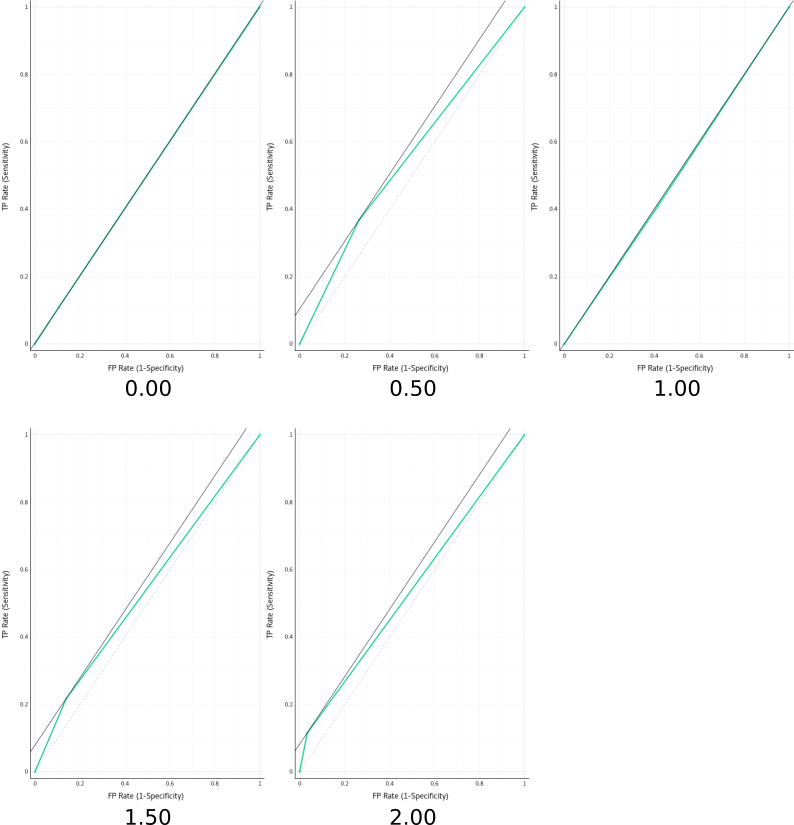
\includegraphics[scale=0.75]{images/roc.png}
% \end{center}
% \caption{Representação gráfica da Curva ROC para cada classe (0.00, 0.50, 1.00, 1.50 e 2.00) induzida no modelo AdaBoost.}
% \label{fig:roc}
% \end{figure}

% O comportamento esperado para a curva, é que a mesma, se aproxime o máximo possível de 1 em cada classe. Entretanto a métrica se apresenta como uma reta nas classes 0.00 e 1.00, nas demais classes tende sutilmente a 1. Conclui-se que a predição das classes 0.00 e 1.00 nos testes estão ocorrendo de forma aleatório pelo classificador.

% Por fim a tabela de contingência ou matriz de confusão, que através da discriminação dos erros ou acertos preditos para cada classe demonstra o desempenho do classificador, uma das métricas mais eficiente de se analisar um classificador. 

% A Tabela ~\ref{tab:matrix_confusion} exibe ao longo da diagonal em tons de cinza as decisões corretas: número de verdadeiros positivos TP e verdadeiros negativos TN; já os elementos fora dessa diagonal representam os erros cometidos: número de falsos positivos FP e falsos negativos FN. É notável que o valor ideal fora da diagonal seja sempre igual a 0.  

% \begin{table}[H]
% \centering
% \begin{tabular}{cc|c|c|c|c|c|c|}
% \cline{3-8}
%  &  & \multicolumn{6}{c|}{\textbf{Predição}} \\ \cline{3-8} 
%  &  & \textbf{0.00} & \textbf{0.50} & \textbf{1.00} & \textbf{1.50} & \textbf{2.00} & $\sum_{}$  \\ \hline
% \multicolumn{1}{|c|}{} & \textbf{0.00} & 4 & 18 & 13 & 2 & 0 & \textbf{37} \\ \cline{2-8} 
% \multicolumn{1}{|c|}{} & \textbf{0.50} & 13 & 42 & 44 & 14 & 1 & \textbf{114} \\ \cline{2-8} 
% \multicolumn{1}{|c|}{} & \textbf{1.00} & 18 & 51 & 78 & 32 & 11 & \textbf{190} \\ \cline{2-8} 
% \multicolumn{1}{|c|}{} & \textbf{1.50} & 7 & 14 & 31 & 15 & 2 & \textbf{69} \\ \cline{2-8} 
% \multicolumn{1}{|c|}{} & \textbf{2.00} & 4 & 2 & 14 & 3 & 3 & \textbf{26} \\ \cline{2-8} 
% \multicolumn{1}{|c|}{\multirow{-6}{*}{\rot{Atual}}} & $\sum_{}$ & \textbf{46} & \textbf{127} & \textbf{180} & \textbf{66} & \textbf{17} & \textbf{436} \\ \hline
% \end{tabular}
% \caption{Tabela de contingência ou Matriz de confusão resultante da indução do classificador AdaBoost.}
% \label{tab:matrix_confusion}
% \end{table}

% \subsection{Considerações Finais}

% E notável que adversidade de classes desbalanceadas influenciou consideravelmente nos resultados preliminares.  A próxima etapa deste estudo merece destaque em uma seção exclusiva para discussão do tema e a análise dos principais métodos na literatura para balanceamento de classes.

% As dificuldades observadas no estudo do problema proposto motivam melhorias e o surgimento de novas estratégias pra a continuidade do trabalho. 

% Os primeiros experimentos realizados na predição, ilustrado no Gráfico abaixo, demonstraram uma taxa de 30\% de acerto na predição da primeira competência exigida em um texto de redação, de uma amostra de 100 redações. 

% A análise gráfica do resultado experimental demonstra que a predição do modelo está em uma faixa especifica de 0.5 a 1.5, ou seja, a indução do modelo deve ser repetida até o mesmo se tornar genérico.

% \pgfplotstableread[col sep=semicolon]{data/adaboost_competence_1.dat}\data
% \begin{figure}[H]
% \begin{center}

% \begin{tikzpicture}
%     \begin{axis}[
%         title=Demonstrar domínio da norma padrão da língua escrita. (1ªCompetência ),
%         width=\textwidth,
%         ymin=0,
%         ytick={0,0.5,1.0,1.5,2.0},
%         ylabel=Pontuação,
%         xtick=data,
%         xticklabel style={rotate=90,anchor=east},
%         xticklabels from table={\data}{title},
%         legend style={ legend columns=-1},
%         enlarge x limits=0.01
%         ]
%         \addplot table[x=id, y=comp1] {\data};
%         \addplot table[x=id, y=adaboost] {\data};
%         \legend{Profissional,AdaBoost}
%     \end{axis}
% \end{tikzpicture}
% \end{center}
% \end{figure}

